%% 
%% Copyright 2007-2020 Elsevier Ltd
%% 
%% This file is part of the 'Elsarticle Bundle'.
%% ---------------------------------------------
%% 
%% It may be distributed under the conditions of the LaTeX Project Public
%% License, either version 1.2 of this license or (at your option) any
%% later version.  The latest version of this license is in
%%    http://www.latex-project.org/lppl.txt
%% and version 1.2 or later is part of all distributions of LaTeX
%% version 1999/12/01 or later.
%% 
%% The list of all files belonging to the 'Elsarticle Bundle' is
%% given in the file `manifest.txt'.
%% 
%% Template article for Elsevier's document class `elsarticle'
%% with harvard style bibliographic references

\documentclass[final,5p,times,twocolumn,authoryear]{elsarticle}

%% For including figures, graphicx.sty has been loaded in
%% elsarticle.cls. If you prefer to use the old commands
%% please give \usepackage{epsfig}

%% The amssymb package provides various useful mathematical symbols
\usepackage{hyperref}
\usepackage{listings}
\usepackage{amssymb}
\usepackage{lipsum}

\lstset{%
  breaklines=true,
  columns=fullflexible,
}

%% The amsthm package provides extended theorem environments
%% \usepackage{amsthm}

%% The lineno packages adds line numbers. Start line numbering with
%% \begin{linenumbers}, end it with \end{linenumbers}. Or switch it on
%% for the whole article with \linenumbers.
%% \usepackage{lineno}

%% You might want to define your own abbreviated commands for common used terms, e.g.:
\newcommand{\kms}{km\,s$^{-1}$}
\newcommand{\msun}{$M_\odot}

\setcitestyle{square}

\begin{document}

\begin{frontmatter}

\title{OpenMPI implementation of Burrows-Wheeler Transform for substring matching applied to genomics}

\author{Andrei S. Blindu}
\affiliation{organization={University of Pavia, Computer Engineering},%Department and Organization
            city={Pavia},
            country={Italy}}

\begin{abstract}
%% Text of abstract
The aim of this project is to provide an efficient parallel implementation of a substring matching algorithm and apply it to the search of genes within the genome of an organism. After implementing the serial algorithm (using C/C++), an a priori study of the available parallelism has been conducted to identify the parts of the code that could be parallelized and then the code has been modified in order to run on multiple CPUs by using OpenMPI. The performance in terms of strong and weak scalability of the parallel implementation have been evaluated by running the code on Google Cloud Platform virtual instances in order to exploit the resources of a cluster of machines. A significant speedup has been obtained compared to the serial version, although under certain conditions the code is not able to scale efficiently as discussed later.
\end{abstract}

\begin{keyword}
Substring Matching \sep Genomics \sep Burrows-Wheeler Transform \sep Parallelization \sep Open MPI \sep Google Cloud Platform
\end{keyword}

\end{frontmatter}

% Table of contents
\tableofcontents

\vspace{\baselineskip}

%% main text

\section{Biological context and Data}
\label{Biological context and Data}
The algorithm considered in this project is being used to find a gene within the genome of an organism. The genome is made up of DNA and contains the set of genes of an organism which are responsible for its traits and characteristics.
DNA is a long double helix molecule composed by a sequence of nucleotides\cite{nucleotide}, each nucleotide is composed by deoxyribose sugar, a phosphate group and a nucleobase. There are four types of nucleobases in DNA: guanine (G), adenine (A), cytosine (C) and thymine (T).
In bioinformatics applications, the genome and the genes are usually considered as long strings of computer code composed by four possible letters (G,A,C,T). \\
The genomes used for this analysis have been taken from the NCBI website\cite{ncbi}. \\
Genomes of different sizes have been used in order to study how the performance changes with respect to the input dataset dimension:
\begin{itemize}
    \item \emph{Escherichia coli}, bacteria commonly found in the lower intestine of warm-blooded organisms\cite{ecoli}, 4.6MB \cite{ecoli dataset}
    \item \emph{Entamoeba invadens}, an amoebozoa parasite of reptiles\cite{entamoeba}, 40.9MB \cite{entamoeba dataset}
    \item \emph{Formica exsecta}, is a species of ant found from Western Europe to Asia \cite{formica}, 277.6MB \cite{formica dataset}
\end{itemize}


\section{Serial implementation}
Having efficient algorithms that allow us to deal with huge genetic sequences is crucial in the bioinformatics field. One of the most used algorithms is the Burrows-Wheeler Transform which was originally intended for data compression but it is used also for string pattern matching problems.

\subsection{Burrows-Wheeler Transform}
The Burrows-Wheeler Transform restructures the original string in a way that is more compressible. It does so by building a matrix whose rows are all the cyclic shifts of the input string, then the rows are lexicographically sorted and finally the last column is selected as the output of the BWT.
Let's consider the following example in Figure \ref{fig:bwt-label} taken from \cite{mreasy}.
\begin{figure}
    \centering
    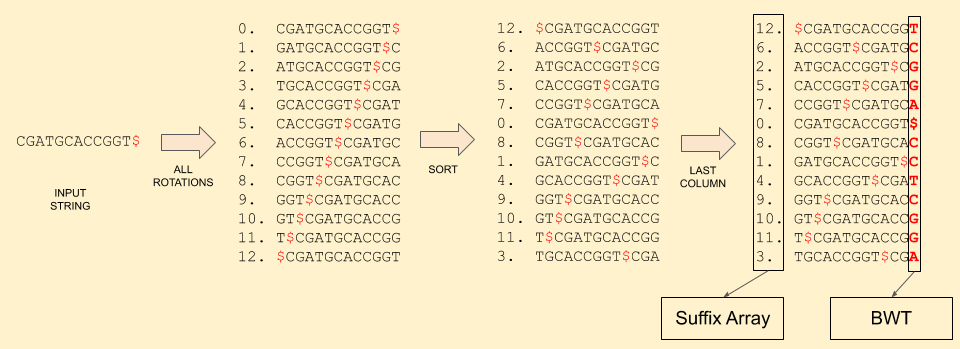
\includegraphics[width=0.5\textwidth]{images/bwt.png}
    \caption{Burrows-Wheeler Transform}
    \label{fig:bwt-label}
\end{figure}
\\ We take the last column (BWT array) because it can be proven that we can recover all the cyclic rotations rows from it and it is the only column having this property that is important to compute the inverse of the transform \cite{geeks}. Moreover, it has better symbol clustering, which means that the same symbols are often grouped together and this favours efficient compression \cite{geeks}. \\
The implementation\cite{bwt.h me} of the Burrows-Wheeler Transform used in this project to compute the BWT array and the Suffix Array for a given genome string has been taken from \cite{geeks}.

\subsection{BWT pattern matching}
After computing the BWT array and the Suffix Array we can use them to efficiently find a pattern (gene) within the genome. The implementation provided in this project\cite{bwt.h me} and described here takes inspiration from \cite{mreasy} and was adapted to our scope using C++ language.\\
As it can be noticed in Figure \ref{fig:bwt-label}, in the first column of the previously computed matrix the nucleobases are sorted and grouped together, so it is possible to compute the bands (range of indexes of the Suffix Array) for all nucleobases. The algorithm starts from the last nucleobase in the pattern and keeps moving towards the start. At first the band of the last nucleobase is computed so we know where to start searching, then the idea is to reduce the band size at each iteration as we move backwards until we eventually either find the starting position of the pattern in the genome or we conclude that no match is found (if the band size reduces to zero before iterating all the pattern string). In order to do so we define a \emph{rank} function that tells how many times a character appeared in the BWT array before a certain index. Then, at each iteration over the nucleobases of the pattern, the start index and end index of the band are updated in the following way:
\begin{lstlisting}[language=c++]
char c = pattern[i];

int rankTop = rank(bwtArr, c, bandStart);
int rankBottom = rank(bwtArr, c, bandEnd);

bandStart = bands[c] + rankTop;
bandEnd = bands[c] + rankBottom;
\end{lstlisting}
If at a certain iteration the start index and the end index of the band coincide it means that the pattern is not found in the genome. Otherwise we find the starting index of the pattern in the genome as the item of the Suffix Array having as index the last value of the start index of the band. 

\subsection{Analysis of the serial algorithm}
In this section, it will be discussed how the serial version of the code has been implemented and the computational costs associated to the different steps of the algorithm, in terms of number of instructions and in relation to the input size. \\
Before applying the previously described BWT algorithm it is necessary to read and preprocess both the genome and the gene file. The path of these files are passed to the \emph{main()} function as parameters when the program is executed. The preprocessing involves removing spaces, new-lines, characters different from the nucleobases symbols, converting lower case letters to upper case and adding a termination character at the end of the preprocessed strings; all these operations are necessary for the correct execution of the algorithm. The computational costs of both the reading and preprocessing are linear with the size of the input file: 
$$ O(genomeSize + patternSize) $$
The Burrows-Wheeler Transform and the pattern matching are implemented in three phases: \\
\begin{enumerate}
    \item \textbf{Suffix Array computation}: as it can be noticed by looking at the code implementation, it contains two for loops iterating over the genome string and an execution of the quicksort algorithm, so the computational cost of this phase can be computed as $$O(2*genomeSize + genomeSize*ln(genomeSize))$$
    \item \textbf{Last column computation}: since it contains basically a for loop iteration over the genome string, its computational cost can be computed as $$O(genomeSize)$$
    \item \textbf{Pattern search}: it iterates the genome string 4 times in order to count the number of occurences for each of the four nucleobases; then assuming we are in the case that a match is found we have to iterate over all the nucleobases in the pattern and for each iteration we have to execute the rank function twice; the cost of the rank computation depends on the index from which we want to count the number of occurences of a character in the BWT array, so on average we can say it is $genomeSize/2$. So we can estimate the total computational cost of the pattern search as
    $$O(4*genomeSize + patternSize*genomeSize)$$
\end{enumerate}
The following table summarizes the computational costs of the different steps. More precise results could be estimated using profiling tools.
\begin{center}
\begin{tabular}{|| c c ||}
\hline
Step & Cost (N. operations) \\
\hline
 Read data & $O(genSize + patSize)$ \\ 
 Preprocess data & $O(genSize + patSize)$ \\  
 Suffix array & $O(2*genSize + genSize*ln(genSize))$ \\
 BWT last column & $O(genSize)$ \\
 Pattern search & $O(4*genSize + patSize*genSize)$ \\
\hline
\end{tabular}
\end{center}

\section{A priori study of available parallelism}
The serial version of the code has been analyzed in order to understand which parts can be parallelized and what enhancement can be theoretically expected by executing the code on multiple CPUs cooperating with each other in parallel.\\
In order to estimate the improvement in performance, in terms of speedup, the \textbf{Amdalh's law} can be used:
$$ Speedup(N) = \frac{1}{S + \frac{P}{N}} $$
Where N is the number of nodes (virtual CPUs) that are exploited, S is the fraction of the code that cannot be parallelized and P is the fraction that can be parallelized. It can be noticed that obviously S+P=1 and the greater is P with respect to S the more speedup is obtained, at least theoretically.\\
In the following analysis parts of the code execution that are less relevant, such as the import of the libraries and the check of the parameters passed to the \emph{main()} function, have been neglected and only the most important blocks, discussed in the previous section, have been considered.\\
The only parts that cannot be parallelized, at least not efficiently or simply, are the reading and preprocessing of the genome and gene files. Even the string matching algorithm based on the Burrows-Wheeler Transform is intrinsically serial, due to loop-carried dependencies, but it is possible to parallelize it by distributing chunks of the genome on different nodes so that the nodes can perform the BWT pattern search in parallel each on a different genome portion, smaller than the whole dataset. The choice of this strategy is also motivated by the fact that, as it can be noticed from the table in the previous section, the computational costs of the operations are highly dependent on the genome dataset size, so we can expect an enhancement by distributing it among different nodes. The methods and issues regarding the parallel implementation will be discussed in greater details in the next section. Whereas it is not possible to distribute the pattern string across different nodes because they all need the whole pattern to be able to find it.\\


\section{OpenMPI parallel implementation}
The parallel version of the code has been developed using OpenMPI (Message Passing Interface) in order to manage different processes running in parallel and their communication on a distributed memory system. In addition to the parameters discussed for the serial implementation, in the parallel version is important to specify the number of CPUs on which to run the program; an error will be generated if the number specified exceedes the capability of the machine or cluster of machines you are running the command on. Moreover, MPI allows to specify an hostfile containing the IP addresses of the machines to execute the code on and the number of slots (virtual CPUs) on each machine; this allows to easily setup a cluster of machines on which to run the tests, as discussed in the next section. \\
The parallel implementation of the code performs the following steps:
\begin{enumerate}
    \item The master reads the genome and pattern files and performs the preprocessing; since these operations are not-parallelizable they are executed only on a single master node.
    \item The master calculates and broadcasts to all slaves the genome size and pattern size. This is important because slaves must know how much memory to allocate before receiving the data in order to avoid segmentation fault errors.
    \item The master broadcasts the pattern to all slaves, after they have allocated the proper amount of memory.
    \item The master splits the genome string in different chunks and sends each slave a chunk and the start index of that chunk with respect to the whole string. The most simple and naive way to perform the splitting is equally divide the genome among the number of nodes. But how can we make sure that genes falling between two different chunks are detected? It can happen that the pattern we are searching for is between two different chunks so if all slaves apply the Burrows-Wheeler search algorithm on its own chunk none is going to find it since none has the whole pattern in its chunk. In order to avoid this nasty problem a simple solution is to have overlapping areas between neighbouring chunks equal to the size of the pattern, so if the pattern is there we make sure it will be detected by at least one of the nodes processing the neighbouring chunks. This solution also takes care of another problem: the integer division of the genome between a finite integer number of nodes leaves out a reminder chunk, but if we suppose that the pattern size is greater than the number of nodes (assumption that is always valid in the experiments performed in this project) then the eventual reminder is covered by extending the chunk size with the pattern size. So each slave allocates memory for the chunks as follows:
    \begin{lstlisting}[language=c++]
    long chunkSize=genomeSize/SIZE;
    long chunkSizeExtended=chunkSize+patternSize;
    char* chunk=(char*)malloc(chunkSizeExtended);
    \end{lstlisting}
    \item Each slave, after receiving its chunk of genome and the start index of that chunk, starts performing the Burrows-Wheeler transform and string matching algorithm with the steps described in the serial version: compute suffix array, compute BWT last column and pattern search. When a node either finds out the position of the pattern in its genome chunk or concludes there's no match prints the result. If there is a match, the position found is summed to the start index of the chunk before being communicated.
\end{enumerate}


\section{Performance and scalability analysis}

\subsection{Fat cluster}
\subsubsection{Intra-regional}
\subsubsection{Infra-regional}

\subsection{Light cluster}
\subsubsection{Intra-regional}
\subsubsection{Infra-regional}


\section{Conclusions}

\begin{thebibliography}{9}
\bibitem{nucleotide} \url{https://en.wikipedia.org/wiki/Nucleotide}
\bibitem{ncbi} \url{https://www.ncbi.nlm.nih.gov/genbank/}
\bibitem{ecoli} \url{https://en.wikipedia.org/wiki/Escherichia_coli}
\bibitem{ecoli dataset} \url{https://www.ncbi.nlm.nih.gov/datasets/taxonomy/562/}
\bibitem{entamoeba} \url{https://en.wikipedia.org/wiki/Entamoeba_invadens}
\bibitem{entamoeba dataset} \url{https://www.ncbi.nlm.nih.gov/datasets/taxonomy/33085/}
\bibitem{formica} \url{https://en.wikipedia.org/wiki/Formica_exsecta}
\bibitem{formica dataset} \url{https://www.ncbi.nlm.nih.gov/datasets/taxonomy/72781/}
\bibitem{geeks}
\url{https://www.geeksforgeeks.org/burrows-wheeler-data-transform-algorithm/}
\bibitem{mreasy} 
\url{https://mr-easy.github.io/2019-12-19-burrows-wheeler-alignment-part-1/}
\bibitem{bwt.h me}
\url{https://github.com/AndreiBlindu/genome-pattern-search-OpenMPI/blob/main/src/utils/bwt.h}
\end{thebibliography}


\end{document}
